\chapter{Pruebas y Resultados pendientes }

\begin{center}
\begin{minipage}{0,6\textwidth}
En este capitulo se presenta los resultados de una serie de pruebas para evaluar el desempeño de la arquitectura de control en tiempo real diseñada para una plataforma abierta de teleoperación.

\end{minipage}
\end{center}








\newpage
%\section{Medición del Ancho de Banda Mecánico del Dispositivo Maestro}
%En la literatura pueden encontrarse varias definiciones de transparencia, la más común es: Un sistema es considerado transparente si las respuestas de posición y fuerza del maestro y del esclavo son idénticas respectivamente, sin importar la dinámica del objeto[]. ii) Un sistema transparente, 
%
%
%
%Para alcanzar una transparencia  aceptable, los dispositivos hápticos cumplir con caracteristicas de baja inercia y no fricción, así como un ancho de banda infinito. Desafortunadamente estas caracteristcas son difíciles de alcanzar y estan relacionadas entre sí, por tanto si se modifica una la otra también se ve a fectada.\\
%
%
%
%
%Al hacer mediciones de corriente en los motores del dispositivo maestro fue necesario implementar una etapa de filtrado ya que como era de esperarse las mediciones de corriente no eran limpias, en algunas ocasiones se encontraban grandes picos en las mediciones.
%
%con la finalidad de no afectar algunas mediciones que parecieran atípicas o de no atenuarlas fue necesario hacer un experimento para encontrar el ancho de banda mecánico del dispositivo, 
%
%
%
%La gráfica del ancho de banda de la articulación del hombro es algo parecido a la siguiente gráfica
%
%As can be seen, the resulting frequency (for -3 dB) is approximately 8 Hz. The current bandwidth is limited by the selected actuator planetary gear. 
%
%\begin{figure}[h!]
%\centering
%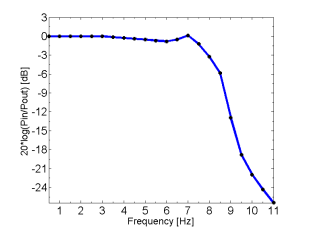
\includegraphics{Figures/MechanichalBandWidth}
%\caption{ALGO ASÍ DEBERÍA RESULTAR DEL ANÁLISIS DEL ANCHO DE BANDA MECÁNICO DEL DISPOSITIVO MAESTRO}
%\label{fig:BandWidth}
%\end{figure}
%








 	
 	

%\section{Estabilidad del Controlador en Corriente}
%El control de corriente fue implementado mediante un bloque PID de LabView, dejando en 0 la ganancia derivativa y usando solo la parte proporcional y la parte integral para corregir el error en estado estacionario
%


%la figura muestra la respuesta del controlador en corriente ante la entrada escalón.
%
%\begin{figure}[htb!]
%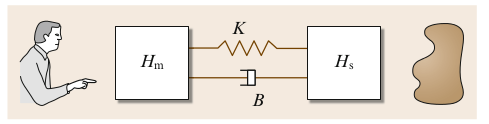
\includegraphics[scale=0.7]{FiguresP/pos-posArq}
%\caption{Diagrama de control fuerza-posición}
%\end{figure}


 	





\newpage
\section{Resultados del Algoritmo Posición-Posición}


\begin{figure}[htb!]
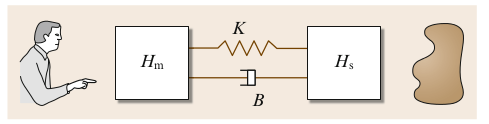
\includegraphics[scale=0.7]{FiguresP/pos-posArq}
\caption{Diagrama de control fuerza-posición}
\end{figure}





\newpage
\section{Resultados del Algoritmo Fuerza-Posición}

\begin{figure}[htb!]
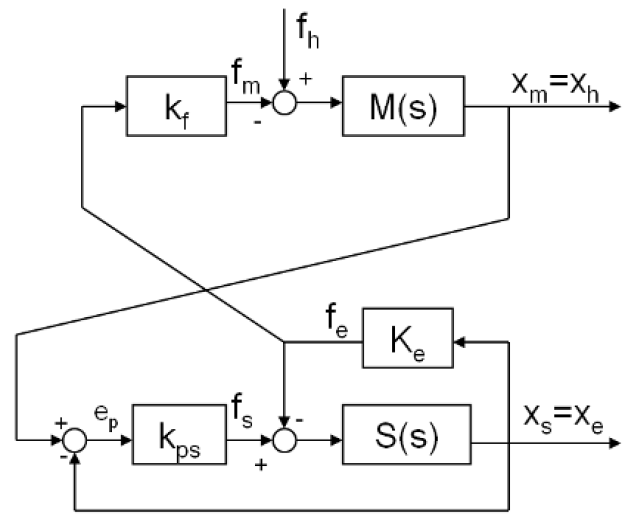
\includegraphics[scale=0.5]{FiguresP/force-pos}
\caption{Diagrama de control fuerza-posición}
\end{figure}


\begin{figure}[htb!]
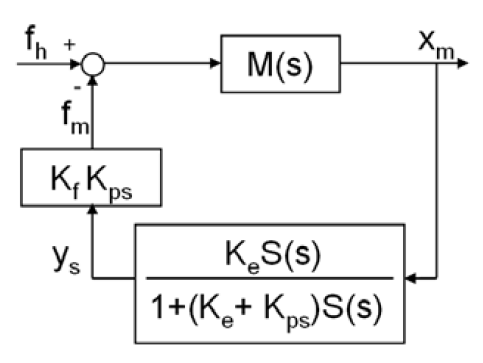
\includegraphics[scale=0.5]{FiguresP/force-pos-operator}
\caption{Diagrama de control fuerza-posición para el  operador}
\end{figure}

Como resultado del algoritmo fuerza posición se espera una menor fuerza ejercida por el esclavo y un menor tiempo de ejecución de una tarea determinada






%\section{Resultados del Algoritmo Híbrido Posición-Fuerza} 	

\section{Resultados ante retardos temporales en el canal de comunicaciones}
con el fin de realizar una prueba para evaluar el comportamiento del sistema ante retardos en el canal de comunicaciones, se introducirá un retardo en la parte del programa de labview que esta encargada de la transmisión y recepción de datos, aumentando gradualmente y evaluando el comportamiento del sistema.







\newpage
\section{Resultados del Tiempo de Ejecución de una Tarea}
Con el fin de evaluar los distintos algoritmos de control se ha diseñado una tarea a realizar por el operador, la tarea consiste en realizar un ensamble de un perno en un orificio, evaluando el tiempo requerido para el ensamble, y las fuerzas ejercidas en el sistema esclavo (ver figura \ref{fig:task}).

%The goal of this task is to push the peg into the hole while avoiding wedging and jamming. The peg has two degrees of motion freedom, hence the dimension of the velocity-controlled subspace is 6 − m = 2, while the dimension of the force-controlled subspace is m = 4. The task frame can be chosen as shown in Fig. 7.3 and the


\begin{figure}
\centering
\label{fig:task}
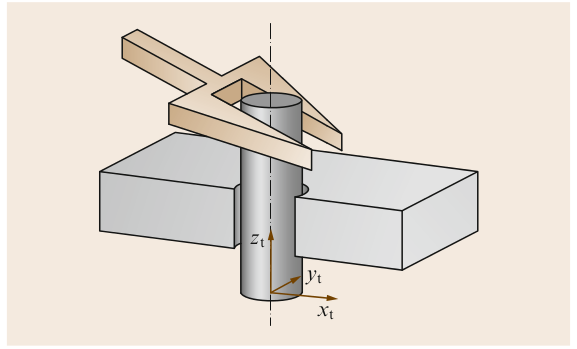
\includegraphics[scale=0.5]{FiguresP/task}
\caption{Tarea propuesta para evaluar la realimentacion de fuerza hacia el operador}
\end{figure}

La tarea de la figura \ref{fig:task} debe ser completada con las siguientes especificaciones de fuerzas y torques. 

\begin{itemize}

\item Fuerzas nulas a lo largo de los ejes $\mathbf{X_t}$ e $\mathbf{Y_t}$

\item Torques nulos alrededor de los ejes $\mathbf{X_t}$ e $\mathbf{Y_t}$

\end{itemize}


Las velocidades obtenidas deben ser:

\begin{itemize}
\item Una velocidad angular diferente de cero a lo largo del eje $\mathbf{Y_t}$

\item una velocidad angular arbitraria alrededor del eje $\mathbf{Z_t}$

\end{itemize}




\begin{figure}
\centering
\label{fig:task2}
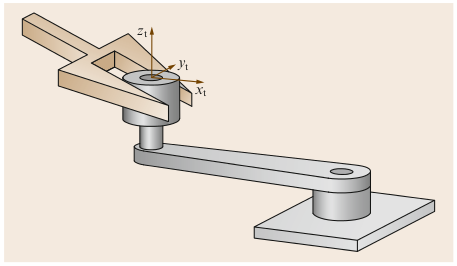
\includegraphics[scale=0.5]{FiguresP/task2}
\caption{Tarea propuesta para evaluar la reflexión de fuerza hacia el operador}
\end{figure}


La tarea de la figura \ref{fig:task2} debe ser completada con las siguientes especificaciones de fuerzas y torques. 


\begin{itemize}

\item Fuerzas nulas a lo largo de los ejes $\mathbf{X_t}$ e $\mathbf{Z_t}$

\item Torques nulos alrededor de los ejes $\mathbf{X_t}$ e $\mathbf{Y_t}$

\end{itemize}


Las velocidades obtenidas deben ser:

\begin{itemize}
\item Una velocidad angular diferente de cero a lo largo del eje $\mathbf{Y_t}$

\item una velocidad angular arbitraria alrededor del eje $\mathbf{Z_t}$

\end{itemize}



comparando los resultados de ambas arquitecturas de control se puede observar los resultados de ambas en tiempo de ejecución de la tarea de prueba y en las fuerzas de contacto ejercidas por el sistema esclavo.\footnote{Al final de las pruebas tenemos que llegar a un resultado parecido al de la figura }



\begin{figure}[htb!]
\centering
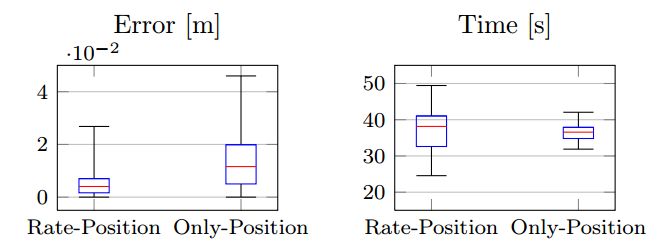
\includegraphics[scale=0.80]{Figures/comparativaAlgoritmos}
\caption{Resultados comparando la implementación de un algoritmo fuerza posición y un algoritmo híbrido fuerza-fuerza, posición-posición}
\label{fig:resultados}
\end{figure}


